\chapter{Prove sperimentali}
\label{chap:prove_sperimentali}
Nei precedenti capitoli è stata presentata l'architettura e il funzionamento del sistema. In questo capitolo vengono analizzati i test del funzionamento del sistema, eseguiti prima sul simulatore e successivamente su un drone reale.

\section{Esperimenti nell'ambiente di simulazione}
La simulazione è uno strumento molto importante nello sviluppo e nell'implementazione di sistemi nel campo della robotica, poiché consente di effettuare esperimenti in un ambiente non reale, controllato e potenzialmente infinite volte, senza costi dovuti al danneggiamento del sistema.
 In particolare, è stato ampiamente utilizzato per verificare il corretto funzionamento dell'algoritmo per la VO e per la missione, prima di fare i test sul drone reale; inoltre, è stato molto utile per comprendere a fondo il firmware PX4 e tutte le sue meccaniche di volo. \\
 
 \subsection{Architettura del sistema}
 L'ambiente simulato è organizzato in tre componenti principali: a simulazione dell'ambiente (World simulation), la simulazione del drone (Drone simulation) e la simulazione della camera a bordo di esso (Onboard camera simulation).
 
 \paragraph{World simulation} Rappresenta l'ambiente nel quale il drone svolge le sue missioni, rispettando il più fedelmente possibile tutte le leggi geometriche e fisiche di un ambiente reale. Inoltre, il mondo simulato avrà al suo interno vari oggetti necessari per l'esperimento, tra cui vari marker ArUco e quattro mura, per simulare lo scenario di un ambiente chiuso. \\
 Il software utilizzato per simulare l'ambiente è Gazebo\footnote{\url{https://gazebosim.org/home}}.
 
 \paragraph{Drone simulation} È il software che si occupa di riprodurre il comportamento reale del drone, simulandone il movimento e le risposte ai comandi. È molto utile per comprendere il funzionamento del firmware PX4 Autopilot, lo stesso che è presente sul flight controller Holybro Pixhawk 6C Mini del drone reale.
  
 \paragraph{Onboard camera simulation} Infine, anche la camera deve essere simulata. In questo caso, essa fa parte di Gazebo. Le immagini vengono prelevate dallo streaming video tramite GStreamer e OpenCV sulla porta UDP 5600 (OpenCV deve essere compilato con il supporto a GStreamer). Le immagini catturate possono essere elaborate dal sistema di visione artificiale utilizzando gli stessi algoritmi della configurazione reale, permettendo dei test più affidabili.
\subsubsection{Parametri}
Il firmware PX4 Autopilot permette di configurare il comportamento del drone, modificandone i suoi parametri\footnote{\url{https://docs.px4.io/main/en/advanced_config/parameter_reference}}. Durante gli esperimenti, sono stati cambiati alcuni di questi parametri dal loro valore di default, per adattarli alle necessità del sistema. In particolare, sono stati modificati i valori relativi al GPS, VO, filtro di Kalman e quelli relativi al movimento. Ecco la lista dei parametri modificati più importanti:
\begin{itemize}
	\item EKF2\_EV\_DELAY = 20.0 ms
	\item EKF2\_EV\_CTRL = 11 (horizontal position, vertical position, yaw) $\rightarrow$ abilità la VO
	\item EKF2\_GPS\_CHECK = 0
	\item EKF2\_GPS\_CTRL = 0
	\item SIM\_GPS\_USED = 0
	\item SYS\_HAS\_GPS = Disable
	\item EKF2\_HGT\_REF = Vision
	\item MPC\_Z\_P = 1.50 $\rightarrow$ è stato aumentato per far alzare il drone con più decisione. La parte di takeoff è una parte critica del volo, dato che il sistema non riesce a vedere marker per un periodo di tempo e rischia di derivare verso una direzione, il che porta a molte problematiche. Facendo alzare il drone con più decisione questo problema viene ampiamente ridotto.
	\item SDLOG\_PROFILE = 131 $\rightarrow$ permette di definire cosa vedere nei file di log.
\end{itemize} 
Un parte fondamentale che merita un approfondimento è come viene calcolato il parametro EKF2\_EV\_DELAY\footnote{\url{https://docs.px4.io/main/en/ros/external_position_estimation\#tuning-EKF2_EV_DELAY}}. Esso corrisponde alla differenza di tempo (in millisecondi) tra la stima della VO e quella dell'IMU, e si può trovare osservando i log. Ad esempio, in Fig. \ref{fig:sim_ev_delay} è rappresentata dalla freccia rossa, e corrisponde a circa 20ms.

\begin{figure}[!htbp]
	\centering
	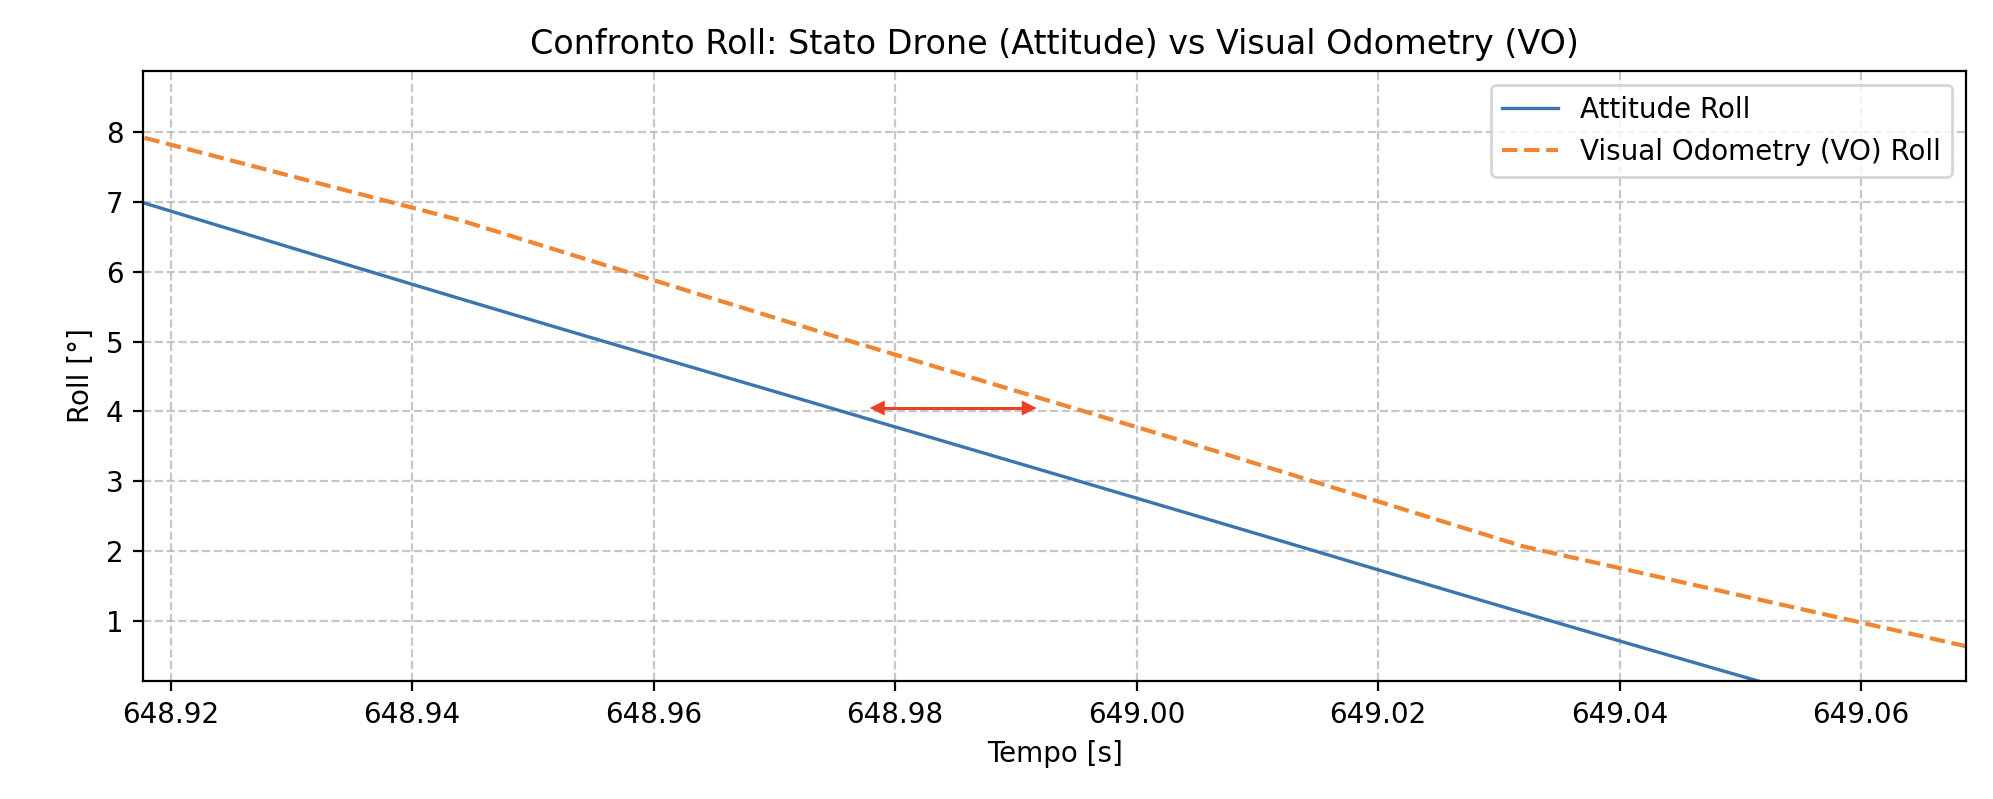
\includegraphics[width = 1\textwidth, trim={0 0 0 0}, clip]{immagini/sim_ev_delay.png}
	\caption{Grafico log del simulatore che confronta il roll della VO e quello dell'IMU per il calcolo del parametro EKF2\_EV\_DELAY.}
	\label{fig:sim_ev_delay}
\end{figure}

\subsubsection{Ambiente}
Il mondo simulato comprende uno scenario contenente 16 marker diversi recintati da dei muri (Fig. \ref{fig:gazebo}). I marker hanno una grandezza di mezzo metro, e sono distanti 2 metri l'uno dall'altro. La distanza e la grandezza dei marker è stata valutata in base al FOV (Field of View) della camera e al tipo di missione da svolgere.\\
La tipologia di drone scelto per l'ambiene simulato è il modello \texttt{gz\_x500\_mono\_cam\_down}\footnote{\href{https://docs.px4.io/main/en/sim_gazebo_gz/vehicles\#x500-quadrotor-with-monocular-camera-down-facing}{\texttt{https://docs.px4.io/main/en/sim\_gazebo\_gz/vehicles\#x500-quadrotor-with-monocular-}\\ \texttt{camera-down-facing}}}. \\
La descrizione json della configurazione dei marker è presente sul github del progetto nel file \path{src/marker_info/aruco_floor_sim.json}; mentre la descrizione del mondo è disponibile nel file \path{my_worlds/aruco_floor.sdf}.
 \begin{figure}[!htbp]
	\centering
	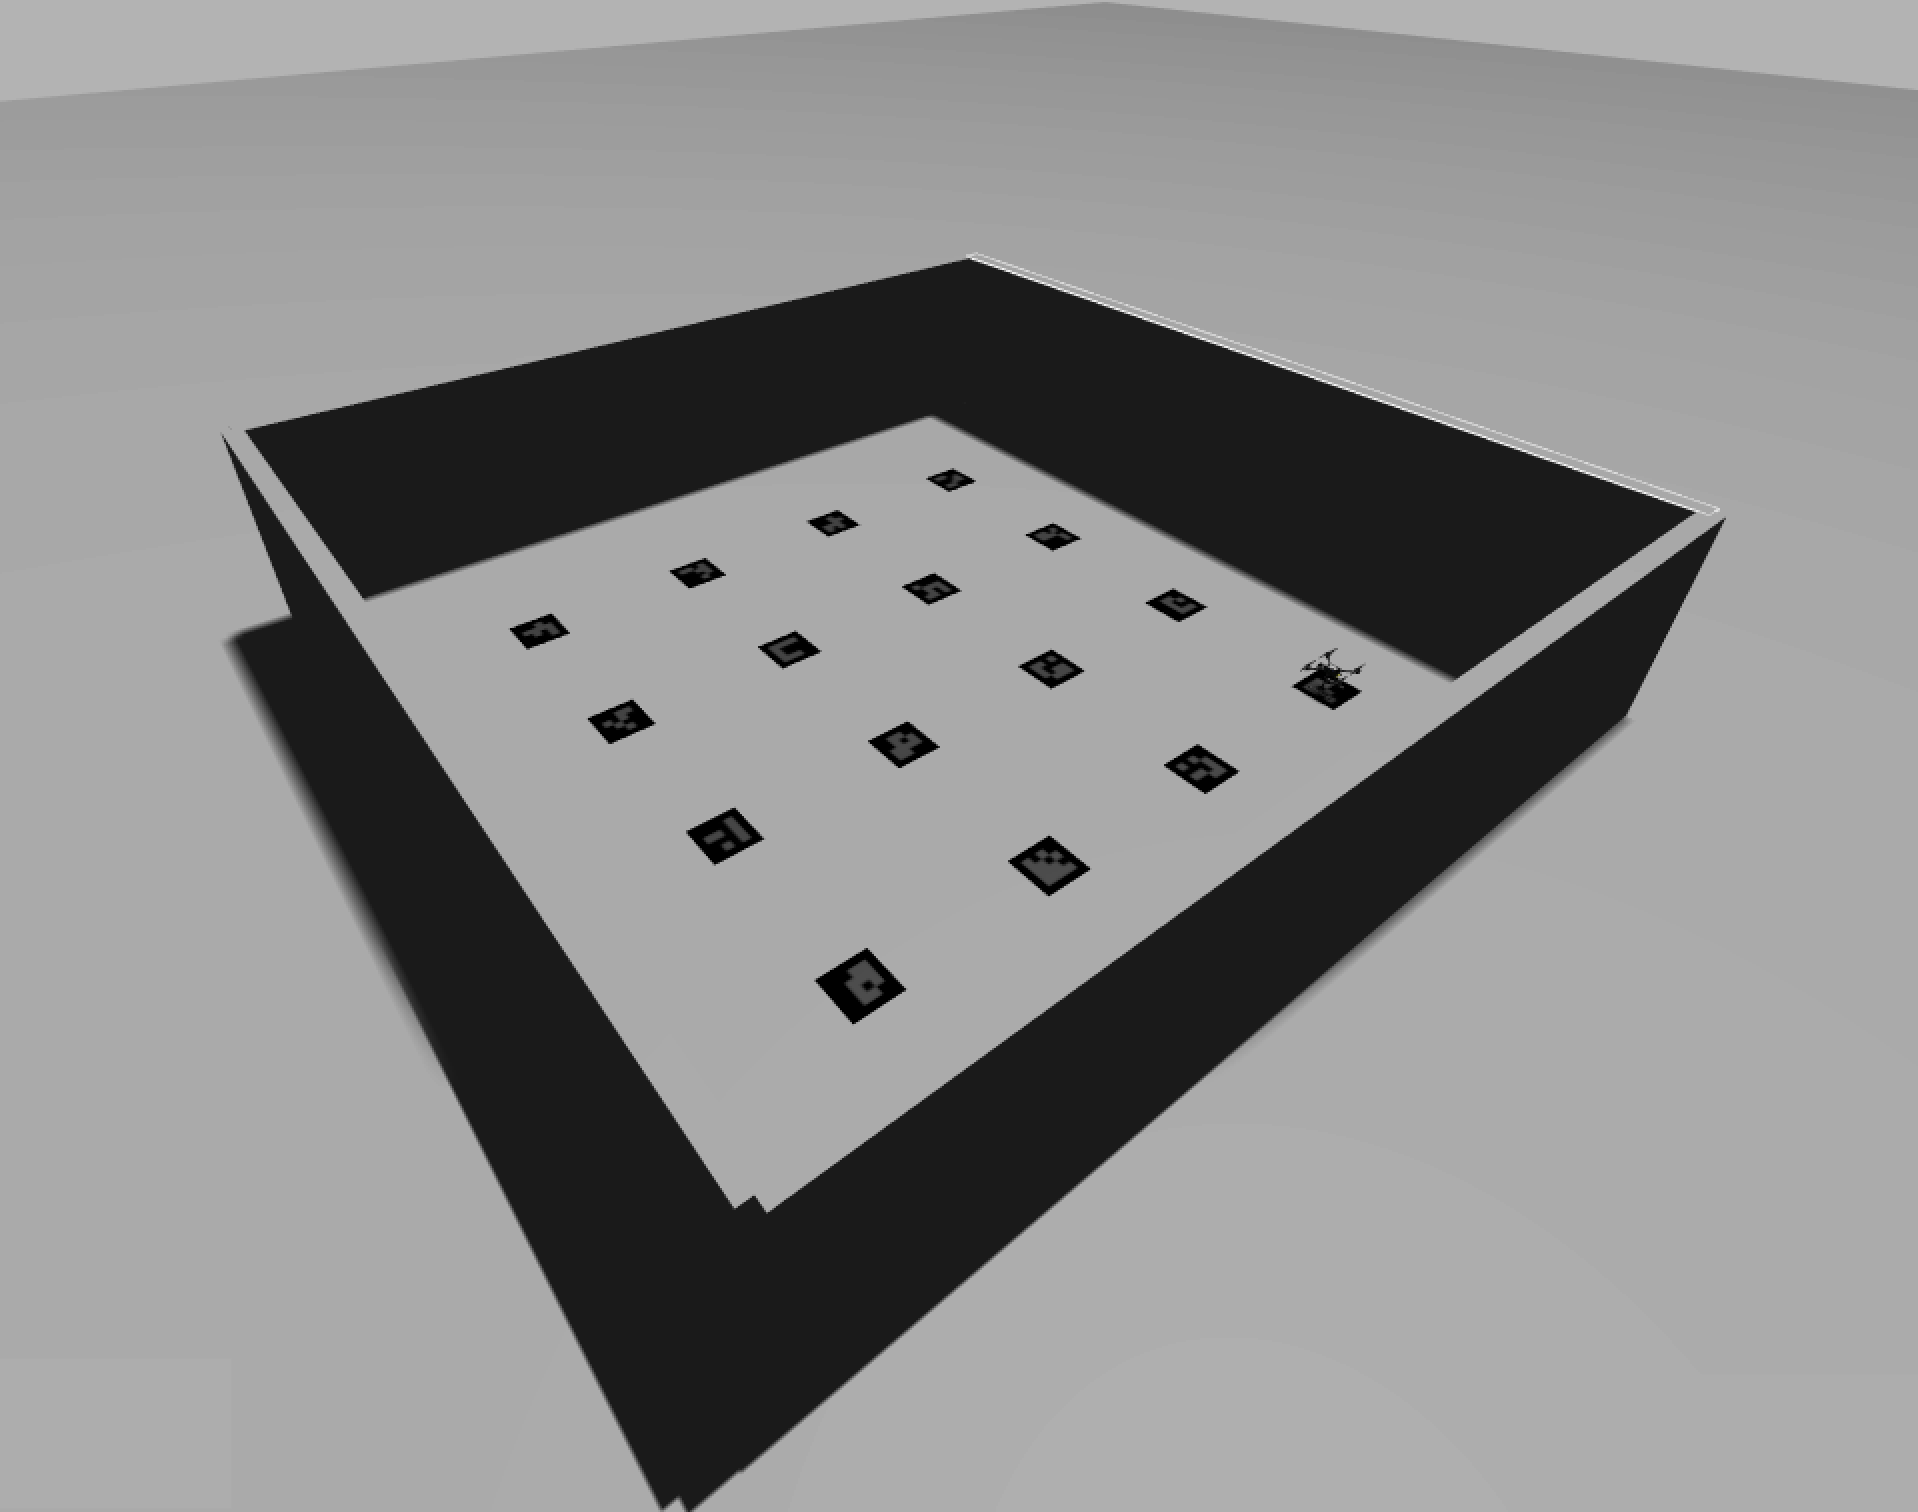
\includegraphics[width=0.7\textwidth, trim={0 0 0 0}, clip]{immagini/gazebo.png}
	\caption{Screenshot del mondo creato dentro Gazebo.}
	\label{fig:gazebo}
\end{figure}

\subsection{Presentazione e analisi dei risultati}
In questa sezione vengono presentati e analizzati i risultati dei test effettuati nell'ambiente simulato. \\
L'analisi si basa principalmente sui file di log che vengono registrati ad ogni sessione di volo. Essi contengono le informazioni relative allo stato del drone, le stime di posizione e posa e i dati che il sistema riceve dalla VO. \\ \\
La missione eseguita e registrata dal log presentata in questa sezione consiste nel raggiungere la posizione NED (4, 2, -1.4) in modalità hoverpoint, partendo dalla (0, 0, -1.4); successivamente, il drone esegue due cerchi grazie alla modalità waypoint; infine, il veivolo ritorna al punto di partenza e atterra. \\ \\
Il log della traiettoria della missione eseguita dal drone è visibile nelle Fig. \ref{fig:sim_xy}, \ref{fig:sim_z}. La traiettoria arancione indica le informazioni inviate al flight controller grazie alla VO; mentre quella blu rappresenta lo stato del filtro di Kalman dopo la fusione dei dati. \\
 \begin{figure}[!htbp]
	\centering
	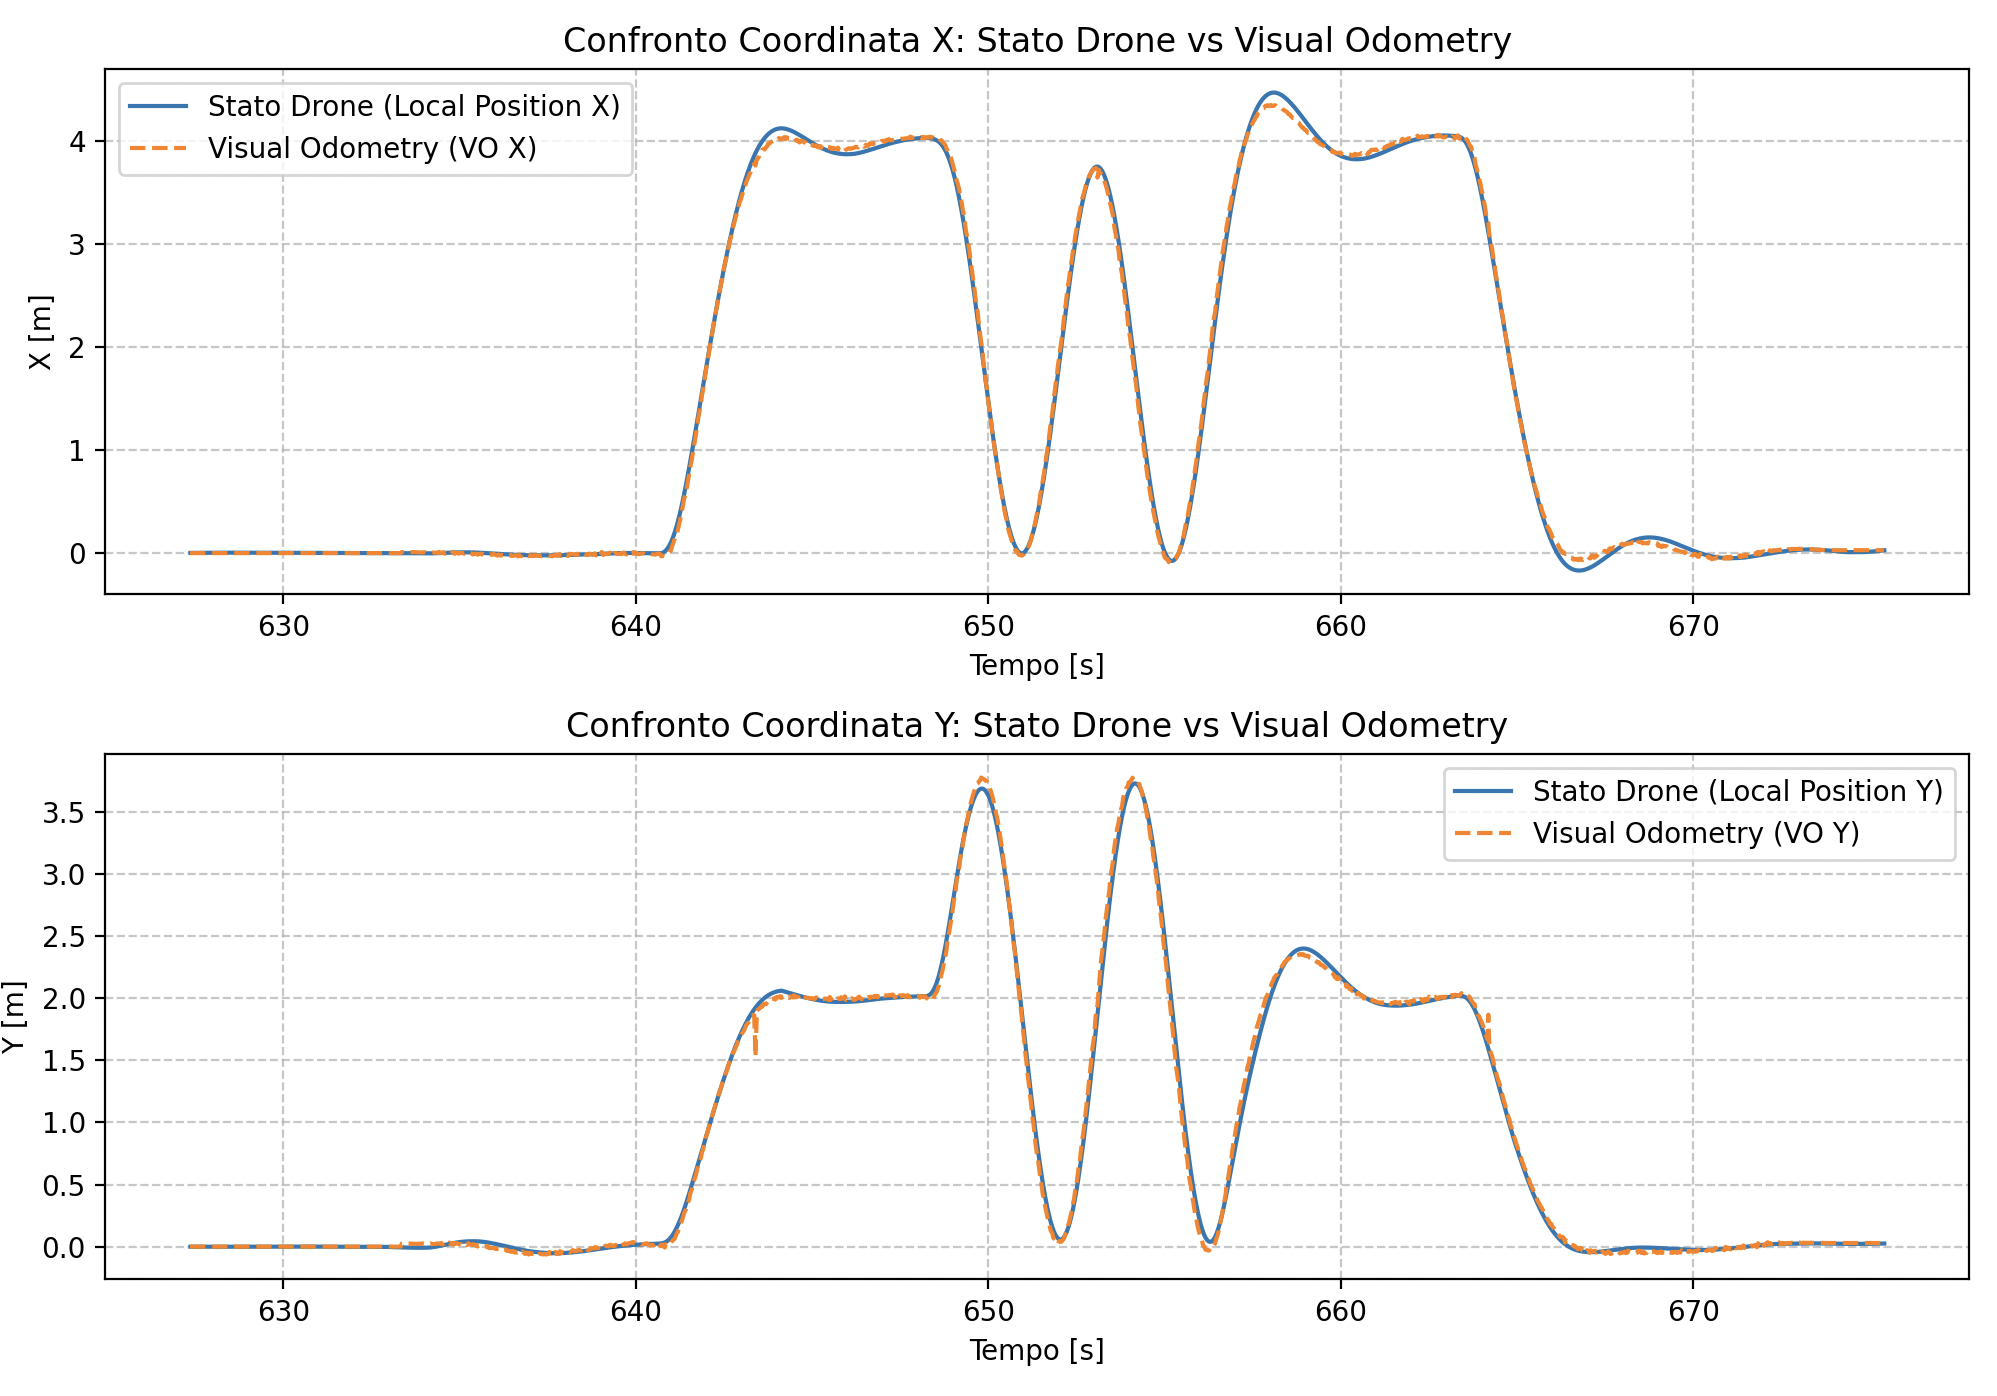
\includegraphics[width=1\textwidth, trim={0 0 0 0}, clip]{immagini/sim_xy.png}
	\caption{Grafico log del simulatore che confronta le coordinate XY della VO e lo stato nel filtro di Kalman.}
	\label{fig:sim_xy}
\end{figure}
 \begin{figure}[!htbp]
	\centering
	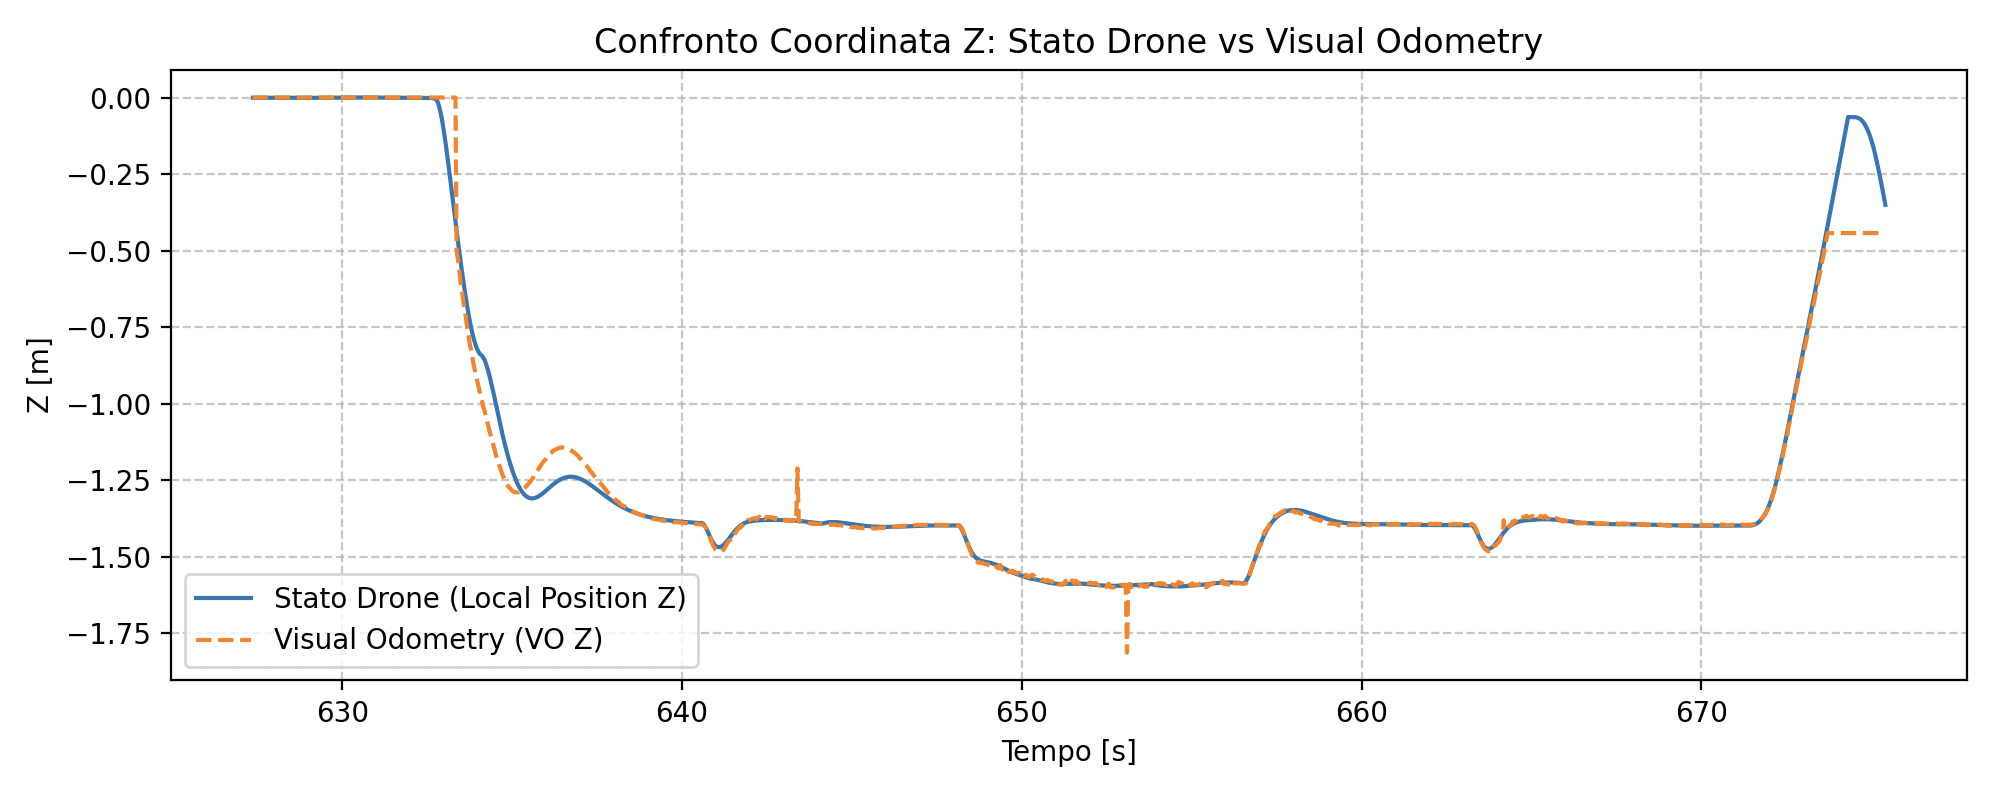
\includegraphics[width=1\textwidth, trim={0 0 0 0}, clip]{immagini/sim_z.png}
	\caption{Grafico log del simulatore che confronta la coordinata Z della VO e lo stato nel filtro di Kalman.}
	\label{fig:sim_z}
\end{figure} \\
Possiamo subito notare come lo stato del filtro di Kalman segua quello della VO, ma non è uguale; questo perchè fa una fusione tra tutti dati, non solo della VO. Inoltre, si può osservare che anche se la VO ha un discostamento anomalo (nelle varie figure se ne possono vedere un paio), il filtro di Kalman corregge questo difetto. \\ 
Per quanto riguarda l'asse Z, possiamo osservare il momento del decollo e di atterraggio. La cosa particolare di queste operazioni è il momento in cui il drone inizia a vedere (o non vede più, in caso di atterraggio) i marker; ma soprattutto anche qui si vede bene il lavoro del filtro di Kalman: nella fase di atterraggio, quando non vede più il marker, di può osservare come la coordinata Z dello stato del drone continua a tendere verso terra; questo avviene grazie alla fusione dei dati con l'IMU. \\
Come spiegato nella Sez. \ref{sec:problema:localizzazione:kalman}, l'IMU anche se correttamente calibrato ha un problema di drift, e qui lo si può notare dal fatto che la coordinata Z non arrivi a 0.\\
Un'ultima considerazione che si può fare è riguardo all'innalzamento dell'altezza del drone, visibile in Fig. \ref{fig:sim_z}: si verificano durante gli spostamenti e una possibile ipotesi di questo effetto è che accade a causa del cambio d'assetto. \\ \\
I log generati dal flight controller non contengono direttamente gli angoli roll, pitch e yaw, ma salvano i quaternioni. Per osservare al meglio i risultati, le Fig. \ref{fig:sim_roll}, \ref{fig:sim_pitch}, \ref{fig:sim_yaw} rappresentano gli angoli convertiti a partire dai quaternioni nel log.\\
Per quanto riguarda i grafici di roll (Fig. \ref{fig:sim_roll}) e pitch (Fig. \ref{fig:sim_pitch}), possiamo notare che i dati della VO e quelli dell'IMU sono praticamente uguali. 
\begin{figure}[!htbp]
	\centering
	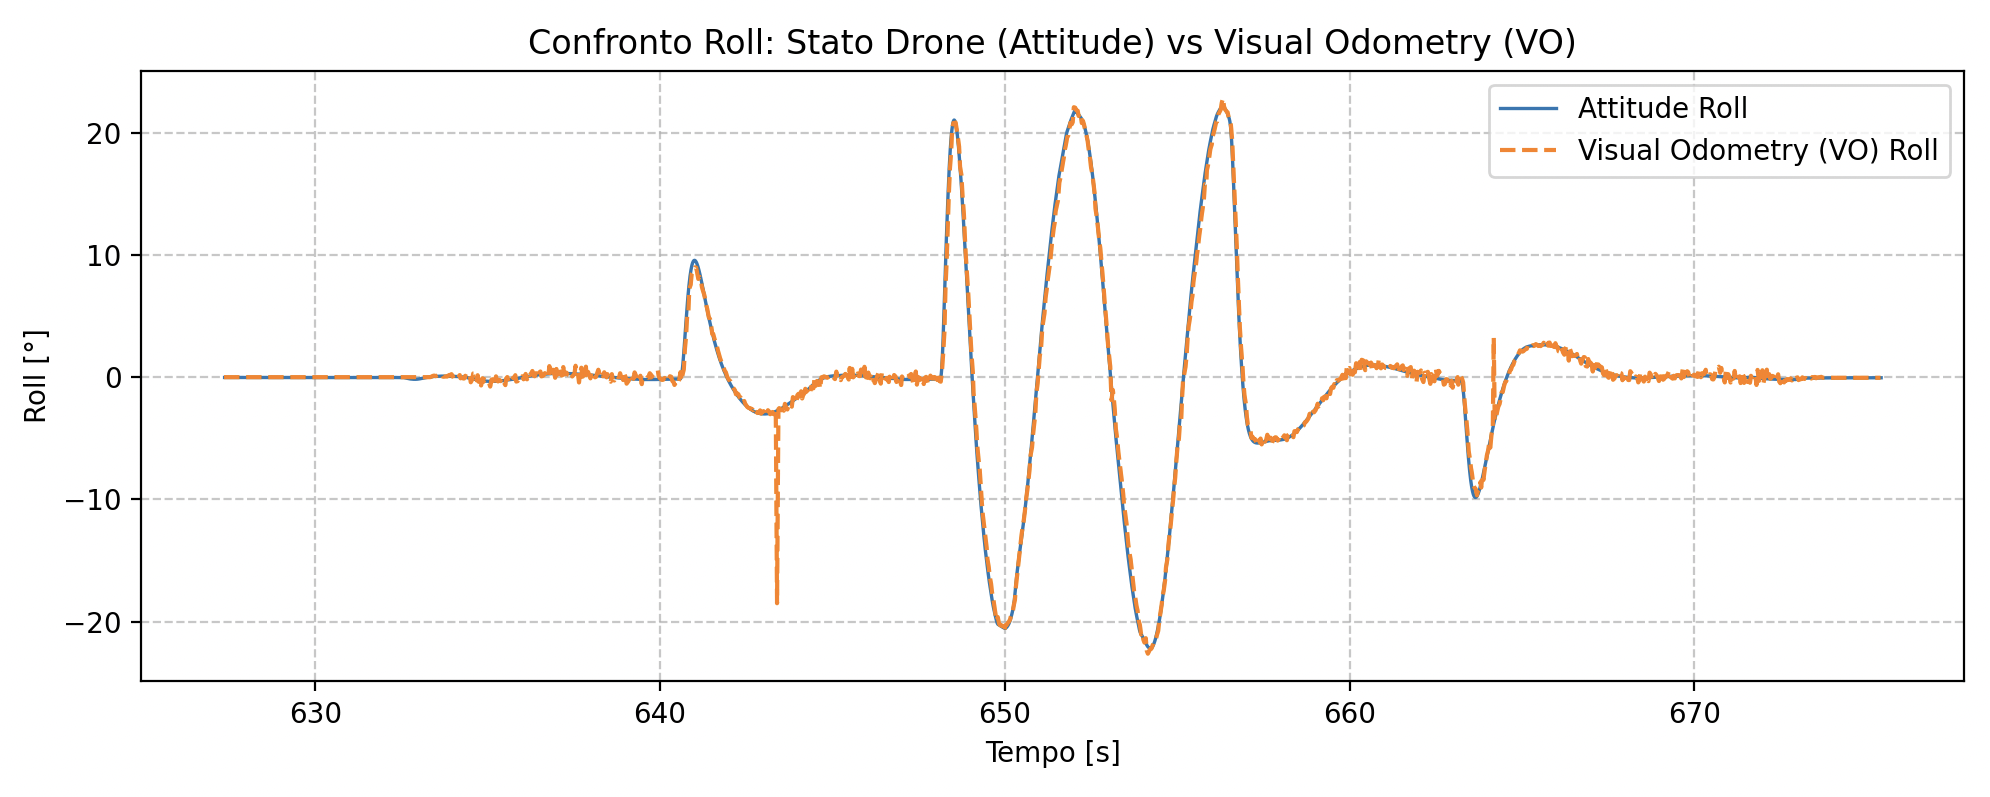
\includegraphics[width = 1\textwidth, trim={0 0 0 0}, clip]{immagini/sim_roll.png}
	\caption{Grafico log del simulatore che confronta il roll della VO e quello dell'IMU.}
	\label{fig:sim_roll}
\end{figure}
\begin{figure}[!htbp]
	\centering
	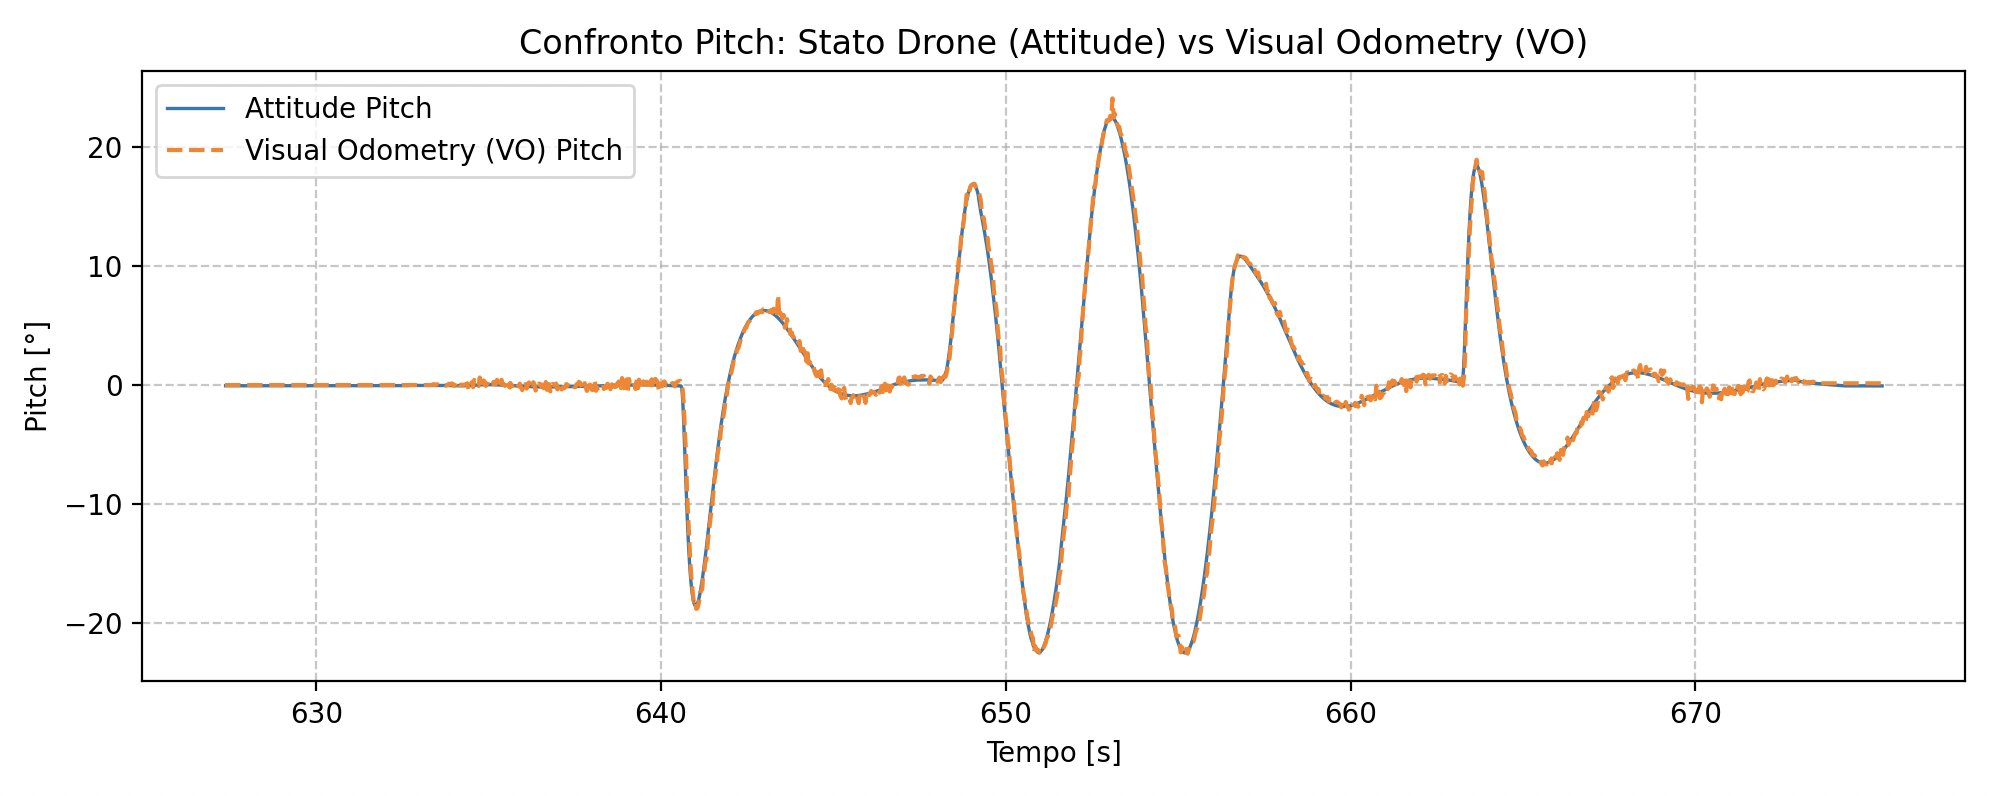
\includegraphics[width = 1\textwidth, trim={0 0 0 0}, clip]{immagini/sim_pitch.png}
	\caption{Grafico log del simulatore che confronta il pitch della VO e quello dell'IMU.}
	\label{fig:sim_pitch}
\end{figure} \\
Un'osservazione importante da fare è che nei grafici si possono osservare delle fluttuazioni rapide, soprattutto quando gli angoli solo vicino allo zero; questo accade perchè risulta molto difficile effettuale il calcolo preciso di questi valori, soprattutto quando la camera di trova perpendicolare al marker. Nonostante ciò, i dati prodotti risultano utilizzabili. \\ \\
I valori dell'angolo yaw generati dalla missione sono osservabili dalla Fig. \ref{fig:sim_yaw}.
\begin{figure}[!htbp]
	\centering
	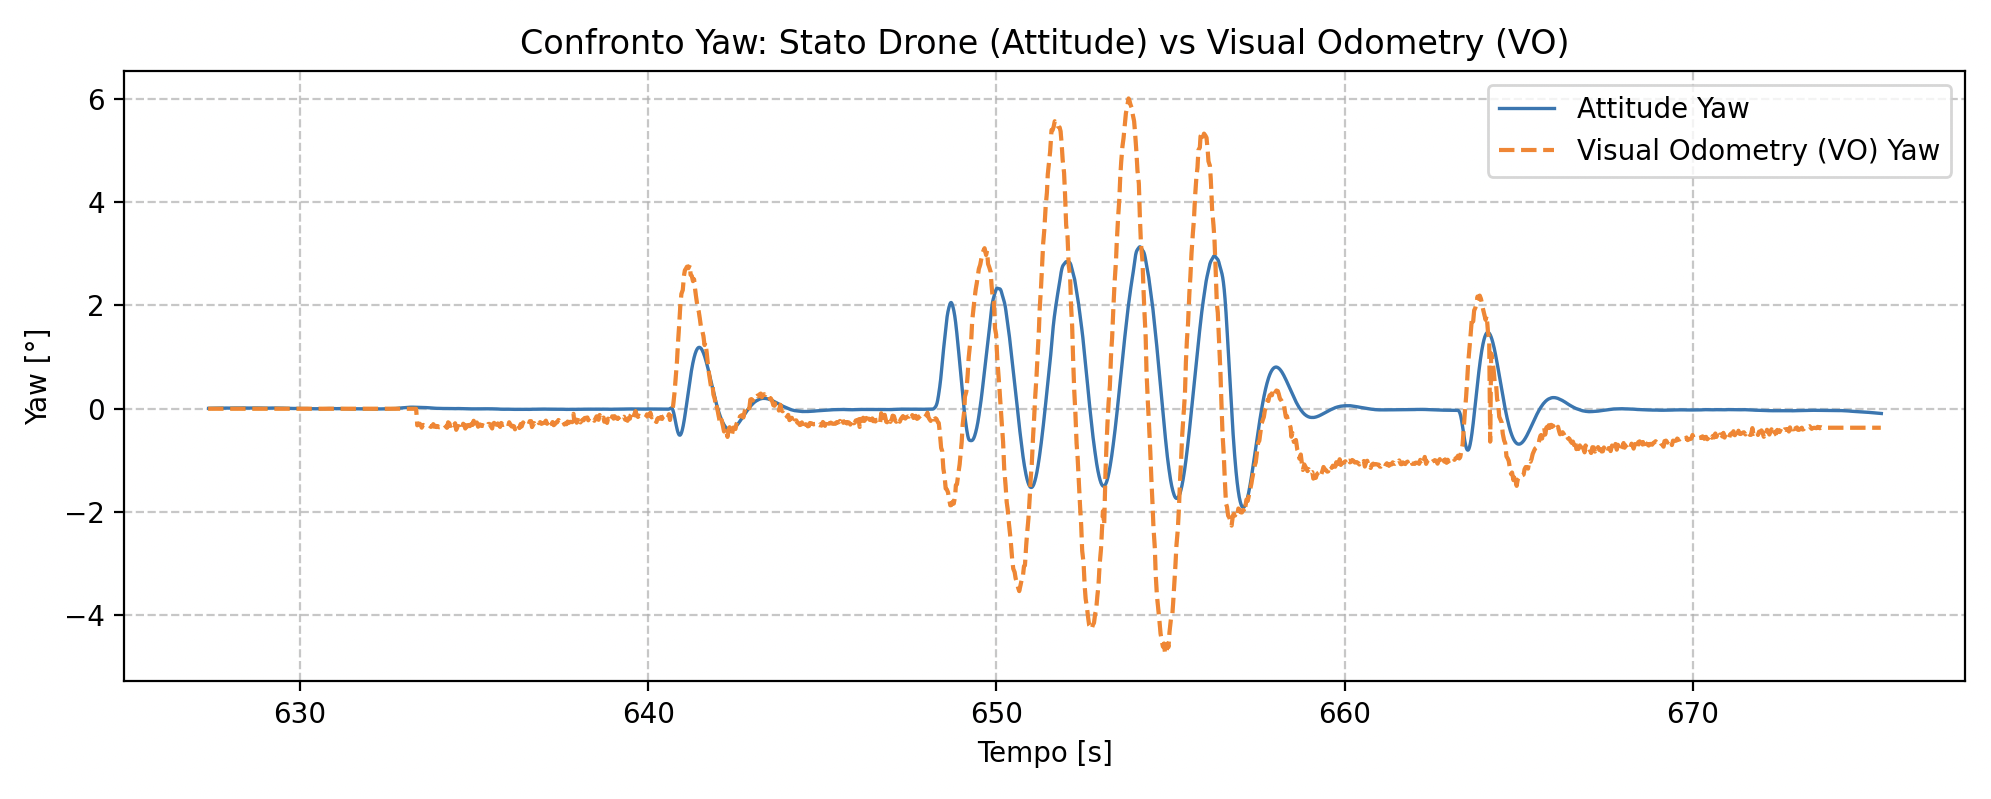
\includegraphics[width = 1\textwidth, trim={0 0 0 0}, clip]{immagini/sim_yaw.png}
	\caption{Grafico log del simulatore che confronta lo yaw della VO e quello dell'IMU.}
	\label{fig:sim_yaw}
\end{figure}\\
Una prima osservazione che possiamo fare è al tempo 634, ovvero al momento in cui il drone inizia a vedere i marker. Anche in questo caso sono presenti le discontinuità notate in precedenza. \\
Si può osservare che sono presenti delle parti in cui i valori dell'IMU non raggiungono la VO. Come nel caso della coordinata Z, questo evento si verifica durante gli spostamenti del drone; quindi, anche in questo caso l'ipotesi è che sia causato dal cambio d'assetto dovuto dallo spostamento del drone. \\ \\
Infine, per quanto riguarda l'esecuzione della missione, il drone è riuscita ad eseguirla senza problemi, volando in modo preciso e deciso, alternando le due modalità di target senza intoppi ed eseguendo le traiettorie dei cerchi in modo accettabile.

\section{Esperimenti di volo reale}
Dopo aver fatto tutte le prove necessarie per costruire il sistema e una volta raggiunto un certo livello di fiducia su di esso, si può passare al test in un ambiente e con un drone reale. In questa sezione vengono descritti ambiente e sistema, seguiti dai risultati ottenuti.

\subsection{Architettura del sistema}
Gli esperimenti con il drone reale sono stati eseguiti utilizzando il sistema hardware presentato nei capitoli precedenti, integrato con i software sviluppati e in parte utilizzati anche negli esperimenti condotti sul simulatore. Rispetto a questi ultimi, il drone fisico introduce ulteriori aspetti legati ai sensori fisici, alle prestazioni del companion computer e all'ambiente.
\subsubsection{Hardware}
Il sistema di volo è costituito da un flight controller Holybro Pixhawk 6C Mini, dotato del firmware PX4 Autopilot, e di un Raspberry Pi 3B, utilizzato come companion computer e incaricato di eseguire i software sviluppati. Quest'ultimo ha installato una camera global shutter OV7251, via connettore CSI del Raspberry; e viene alimentato attraverso un modulo step-down adeguato, che abbassa la tensione dai 14.8V nominali della batteria ai 5V necessari al Raspberry. Per finire, la comunicazione tra flight controller e companion computer avviene via seriale attraverso il protocollo MAVLink 
\subsubsection{Parametri}
Come già visto nel caso del simulatore, anche nel drone reale si devono cambiare alcuni dei parametri di default, per poter utilizzare il sistema correttamente. Qui sono elencati quelli più importanti:
\begin{itemize}
	\item EKF2\_EV\_DELAY = 160.0 ms
	\item EKF2\_EV\_CTRL = 11 (horizontal position, vertical position, yaw) $\rightarrow$ abilità la VO
	\item EKF2\_GPS\_CHECK = 0
	\item EKF2\_GPS\_CTRL = 0
	\item SYS\_HAS\_GPS = Disable
	\item EKF2\_HGT\_REF = Vision
	\item MPC\_Z\_P = 1.50 $\rightarrow$ anche in questo caso è stato aumentato per far alzare il drone con più decisione, e quindi diminuire il difetto di non riuscire a trovare il marker in fase di decollo.
	\item SDLOG\_PROFILE = 1155 $\rightarrow$ permette di definire cosa vedere nei file di log.
\end{itemize} 
Il calcolo del parametro EKF2\_EV\_DELAY è stato eseguito con lo stesso metodo di prima, eseguendo una media dei valori trovati. \\
Infine, a differenza del simulatore, nel drone reale è necessario calibrare tutti i sensori per ottenere dei risultati più precisi, anche più di una volta. Questo accade perchè sensori come l'IMU tendono a scalibrarsi con il passare del tempo e dell'uso.

\subsubsection{Ambiente}
Gli esperimenti sono stati eseguiti dentro un magazzino al chiuso, utilizzando nove marker diversi. I marker hanno una grandezza di 18.5 centimetri, distanti 80 centimetri l'uno dall'altro. Come nel simulatore, anche nel test reale le distanze e la grandezza dei marker sono state scelte in base ai componenti utilizzati nel sistema e al tipo di missione da eseguire. Una foto dell'ambiente è disponibile nella Fig. \ref{fig:magazzino}. \\
La descrizione dei marker è presente nel file \path{src/marker_info/aruco_floor.json}.
\begin{figure}[!htbp]
	\centering
	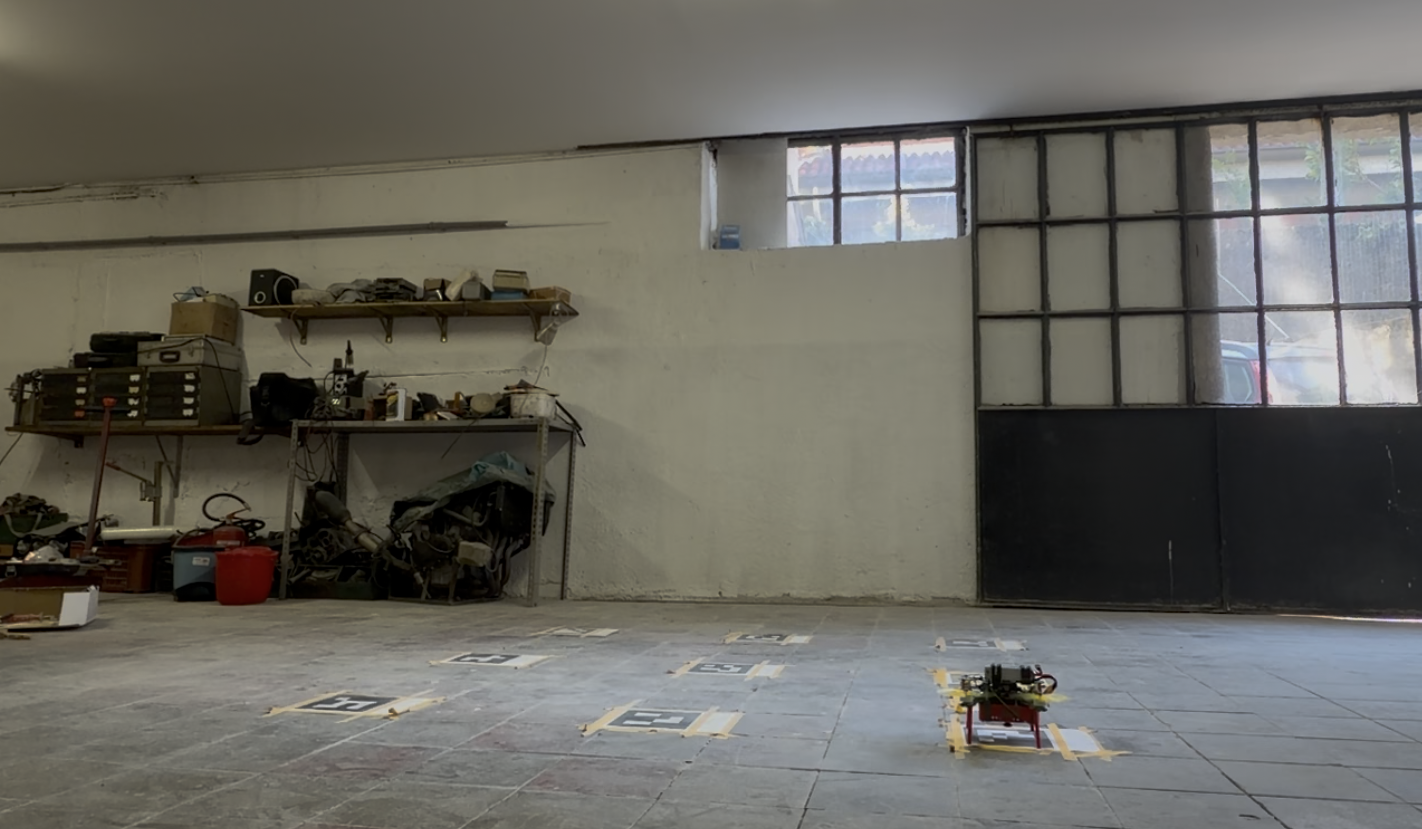
\includegraphics[width = 0.75\textwidth, trim={0 0 0 0}, clip]{immagini/magazzino.png}
	\caption{Foto scattata dentro l'ambiente dove sono stati fatti i test con il drone reale.}
	\label{fig:magazzino}
\end{figure}

\subsection{Presentazione e analisi dei risultati}
In questa sezione vengono presentati i risultati ottenuti durante le prove di volo reale, con l'obiettivo di valutare il funzionamento di tutto il sistema nella realtà dopo le prove fatte al simulatore. \\
L'analisi si basa sul confronto tra la VO inviata dal companion computer e i dati che il flight controller registra\\ \\
Analizziamo i valori di roll e pitch, visualizzabili dalle Fig. \ref{fig:real_roll}, \ref{fig:real_pitch}.
\begin{figure}[!htbp]
	\centering
	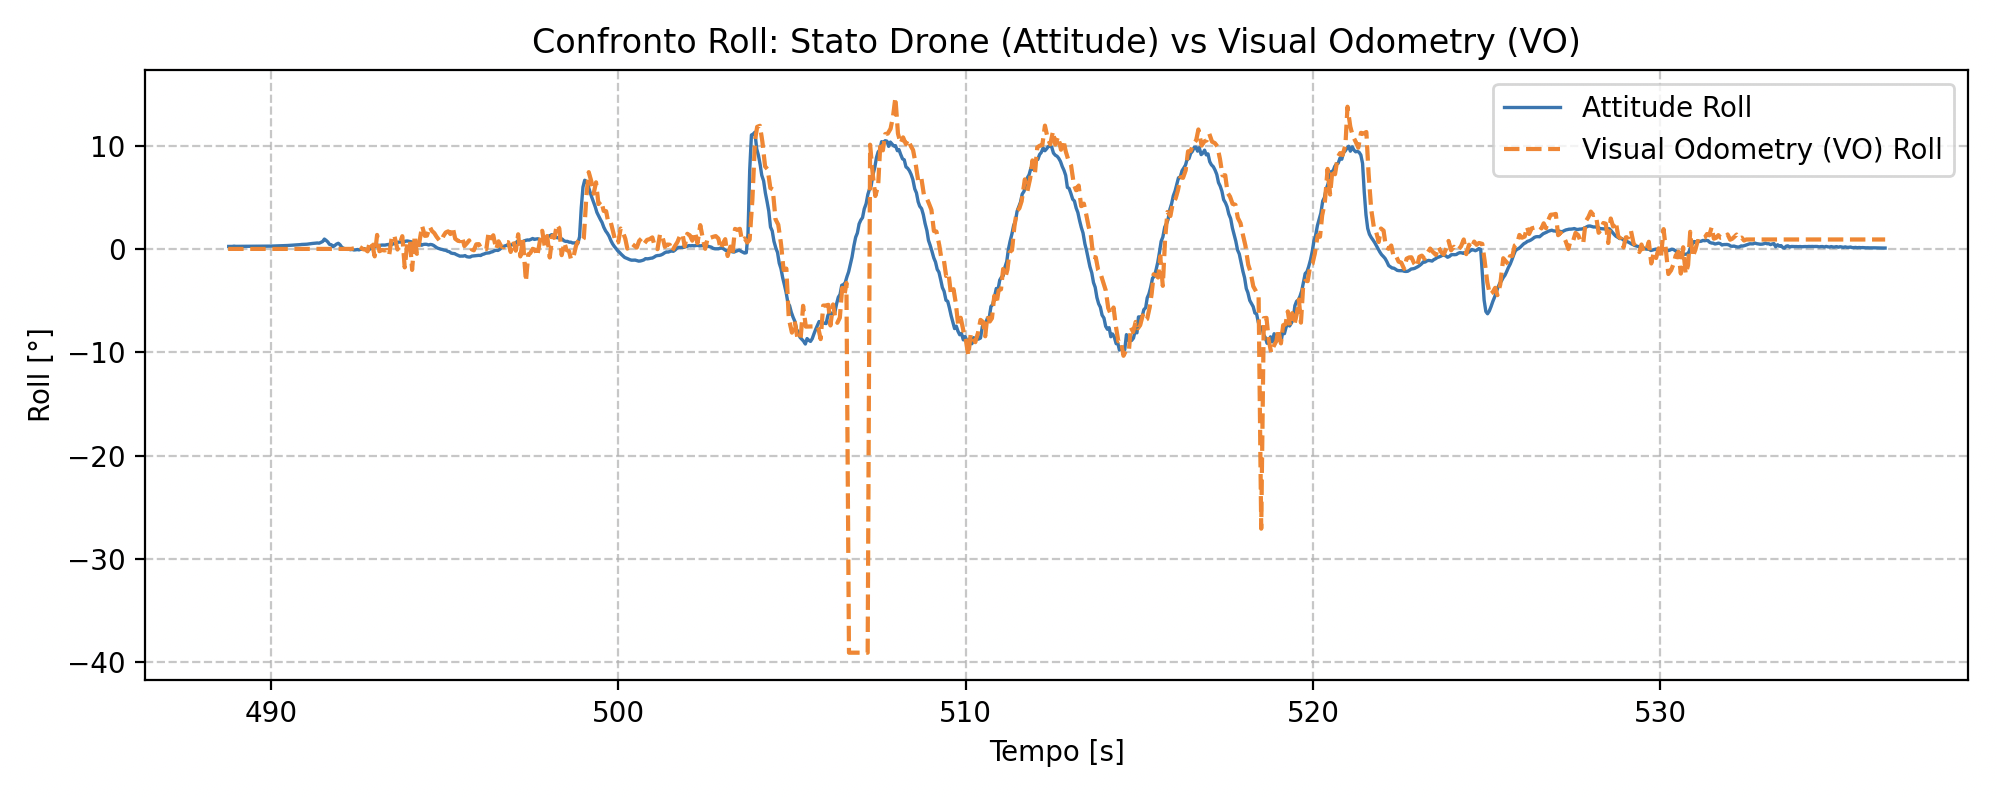
\includegraphics[width = 1\textwidth, trim={0 0 0 0}, clip]{immagini/real_roll.png}
	\caption{Grafico log di volo reale che confronta il roll della VO e quello dell'IMU.}
	\label{fig:real_roll}
\end{figure}
\begin{figure}[!htbp]
	\centering
	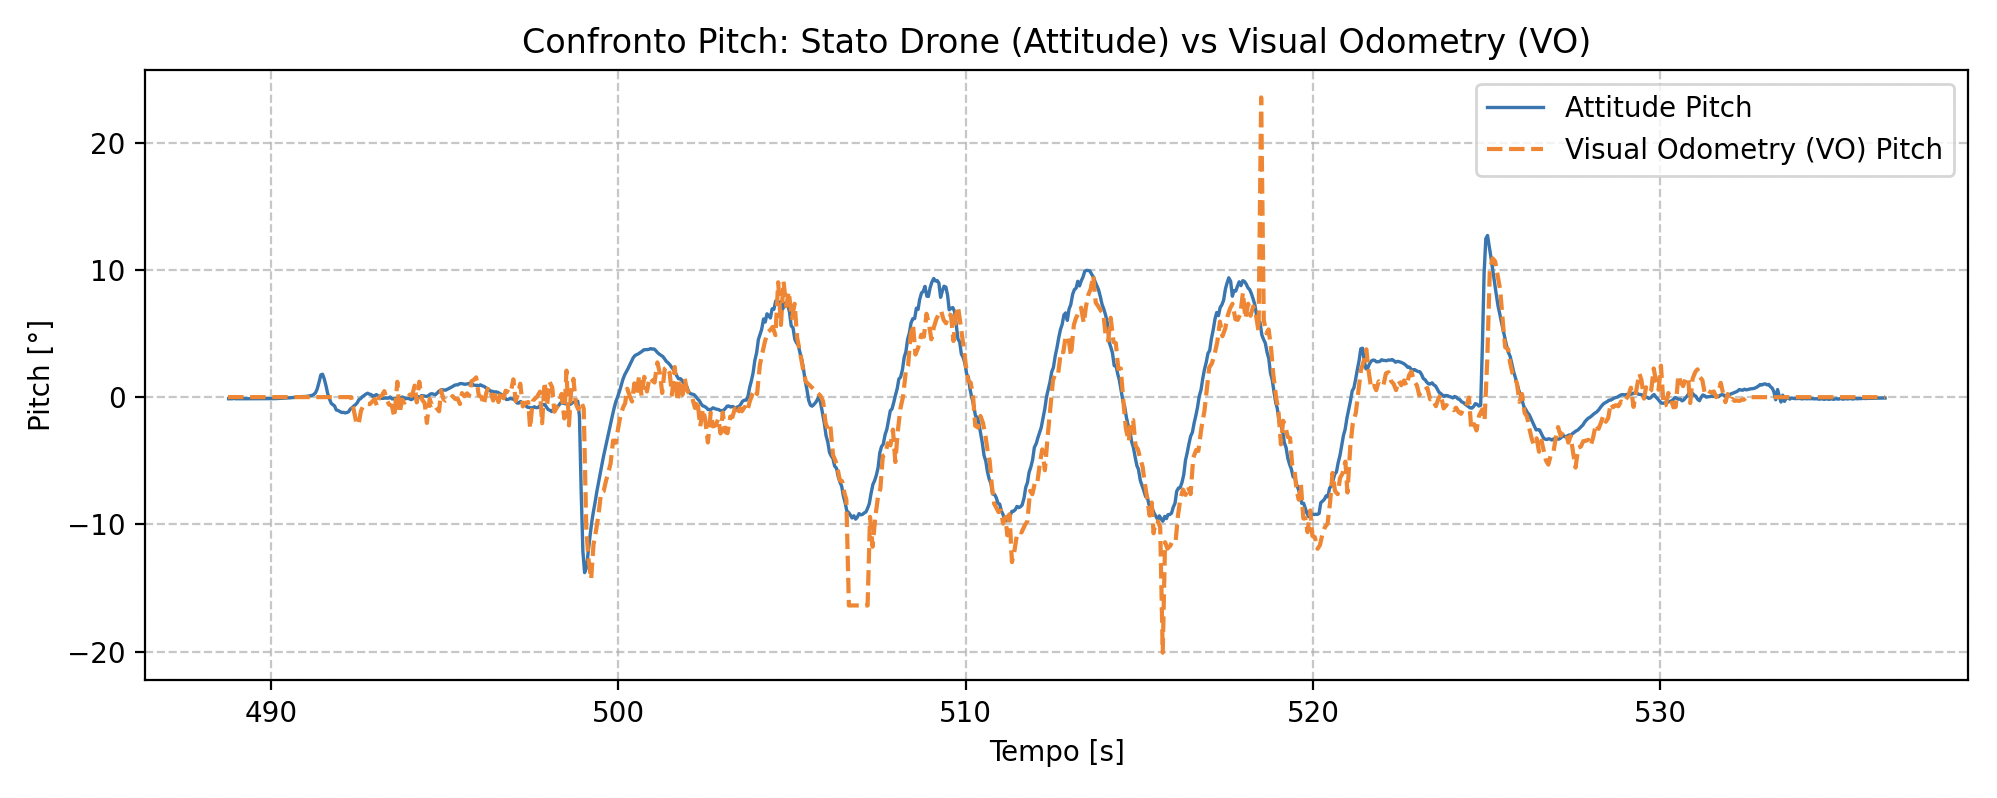
\includegraphics[width = 1\textwidth, trim={0 0 0 0}, clip]{immagini/real_pitch.png}
	\caption{Grafico log di volo reale che confronta il pitch della VO e quello dell'IMU.}
	\label{fig:real_pitch}
\end{figure}
Possiamo osservare che i valori di IMU e VO si inseguono a vicenda; il problema sono le fluttuazioni rapide riscontrate anche nel simulatore. Nel drone reale, queste fluttuazioni sono più accentuate e causano delle instabilità nel volo. Nella Fig. \ref{fig:real_probl} è presente uno zoom del grafico di roll, e si possono notare questa variazioni di circa 2°, che per i valori di roll e pitch sono abbastanza per far muovere il drone. Sono stati registrati casi in cui queste variazioni erano superiori.
\begin{figure}[!htbp]
	\centering
	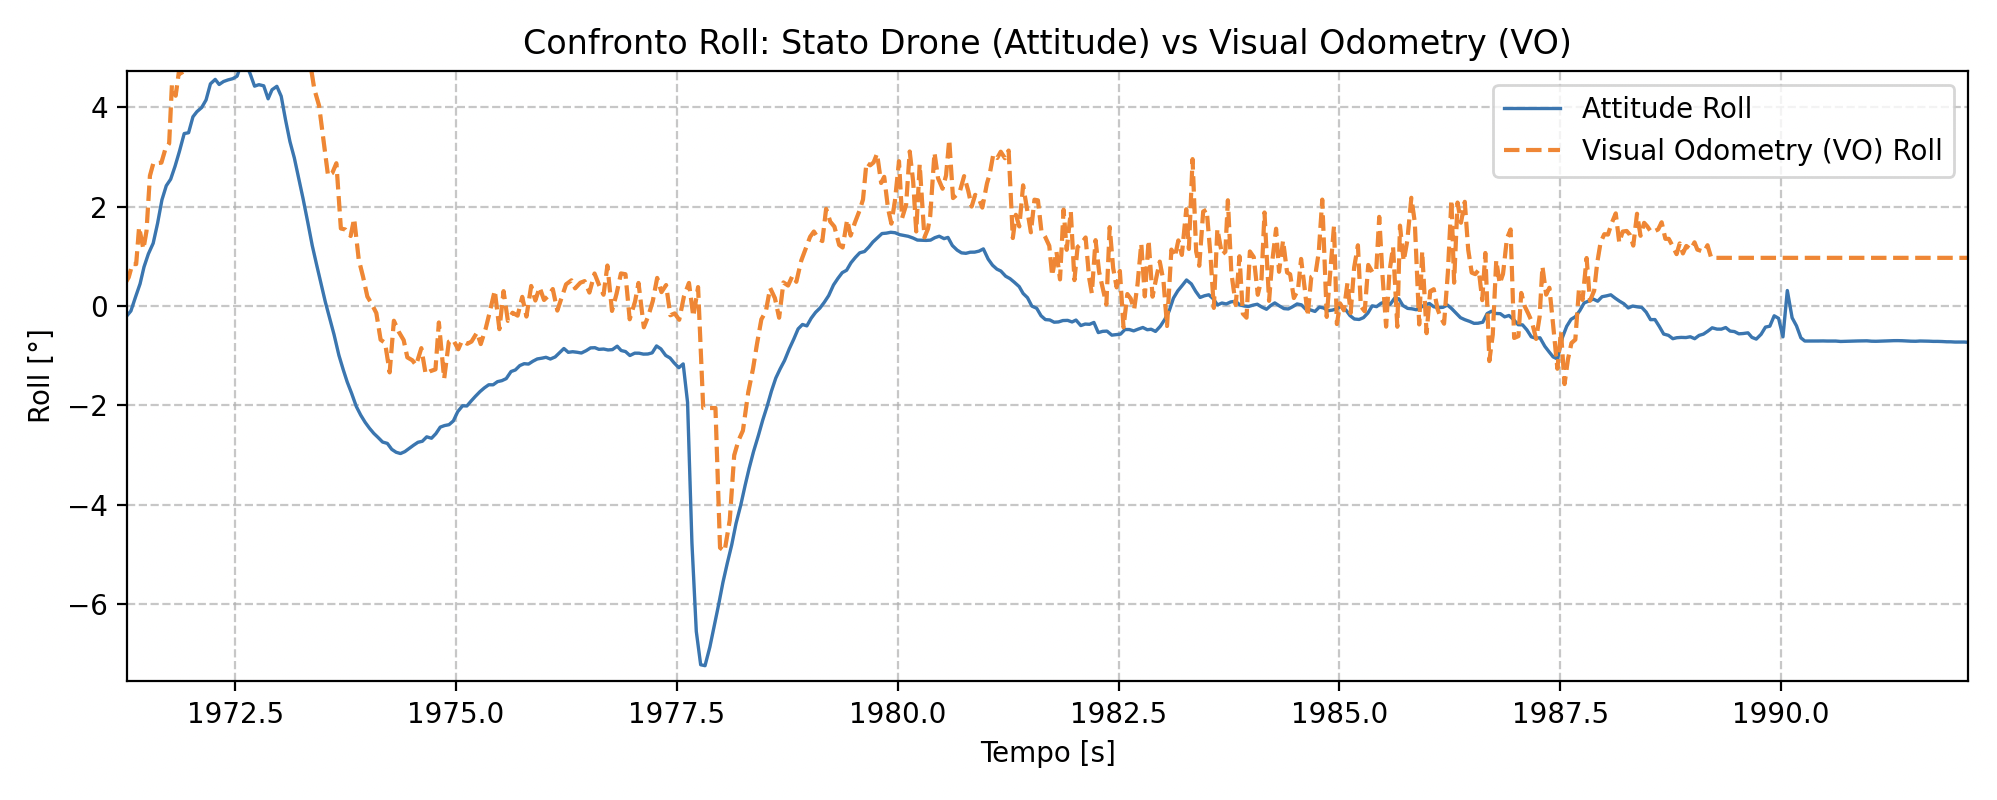
\includegraphics[width = 1\textwidth, trim={0 0 0 0}, clip]{immagini/real_probl.png}
	\caption{Grafico log di volo reale che mostra il problema del calcolo di roll e pitch con la VO.}
	\label{fig:real_probl}
\end{figure} \\
Per questo motivo è stato scelto di escludere i valori di roll e pitch dalla VO, e affidare il calcolo di questi valori all'IMU che, se correttamente calibrato, rappresenta un ottimo stimatore per questi valori; inoltre, non risulta più necessario avere la camera perfettamente perpendicolare al flight controller. Per fare ciò, basta inserire nella matrice di covarianza il valore \texttt{NaN} nelle posizioni in cui il calcolo della VO non è valido\footnote{\url{https://mavlink.io/en/messages/common.html\#ODOMETRY}}. \\ \\
Lo yaw risulta molto valido. In questo caso, è necessario che il filtro di Kalman lo elabori dato che l'IMU stima lo yaw tramite gli accellerometri; e inoltre, in questo modo lo yaw dipende dall'orientamento dei marker, non da quello iniziale del drone. Nella Fig. \ref{fig:real_yaw} è preente il grafico dello yaw di questa missione. Osservando l'asse Y, possiamo notare che lo yaw oscilla di 3-4°, valori perfettamente normali, soprattutto quando il drone è in movimento. 
\begin{figure}[!htbp]
	\centering
	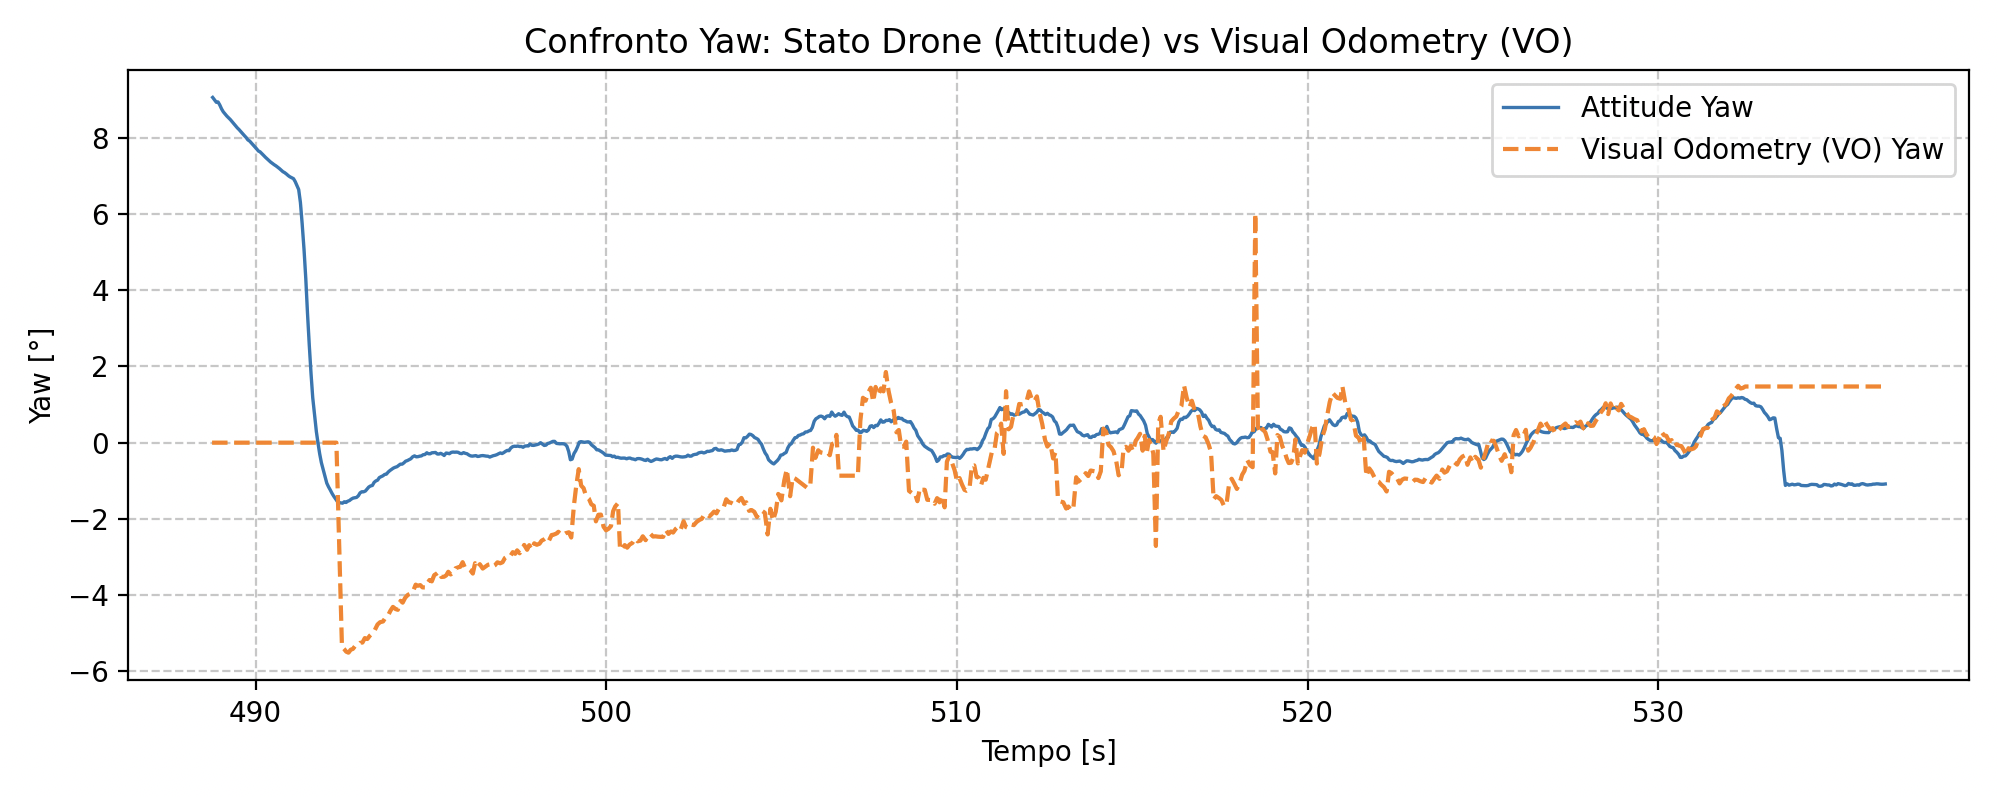
\includegraphics[width = 1\textwidth, trim={0 0 0 0}, clip]{immagini/real_yaw.png}
	\caption{Grafico log di volo reale che confronta lo yaw della VO e quello dell'IMU.}
	\label{fig:real_yaw}
\end{figure}
La Fig. \ref{fig:real_yaw2} mostra lo yaw di un volo eseguito in manuale, utilizzando sempre lo stesso sistema per la VO. Qui si può facilmente notare come entrambi i valori si comportino allo stesso modo; inoltre, al tempo 54 è presente una discontinuità dovuta dal fatto che il dominio di yaw è [-180°, 180°].
\begin{figure}[!htbp]
	\centering
	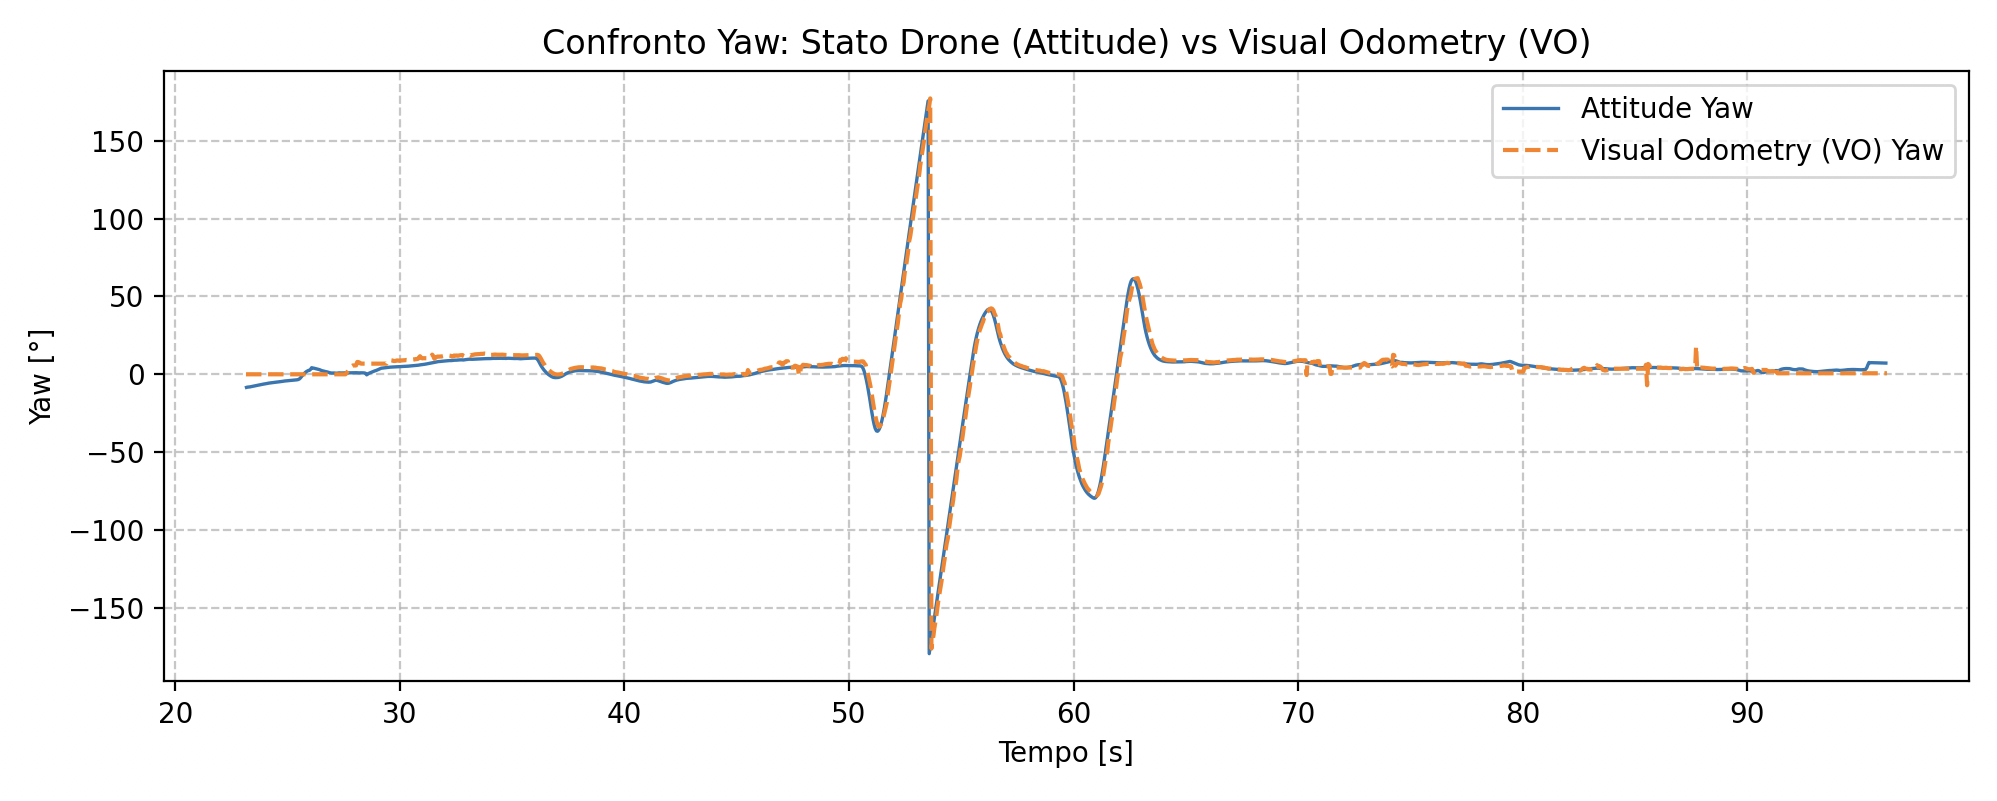
\includegraphics[width = 1\textwidth, trim={0 0 0 0}, clip]{immagini/real_yaw2.png}
	\caption{Grafico log di volo reale in modalità manuale che confronta lo yaw della VO e quello dell'IMU.}
	\label{fig:real_yaw2}
\end{figure} \\
Per quanto riguarda il calcolo della posizione, nella Fig. \ref{fig:real_xy} si può osservare come le coordinate X e Y siano ottime: il filtro di Kalman segue correttamente i dati della VO, correggendo le eventuali fluttuazioni temporanee. 
\begin{figure}[!htbp]
	\centering
	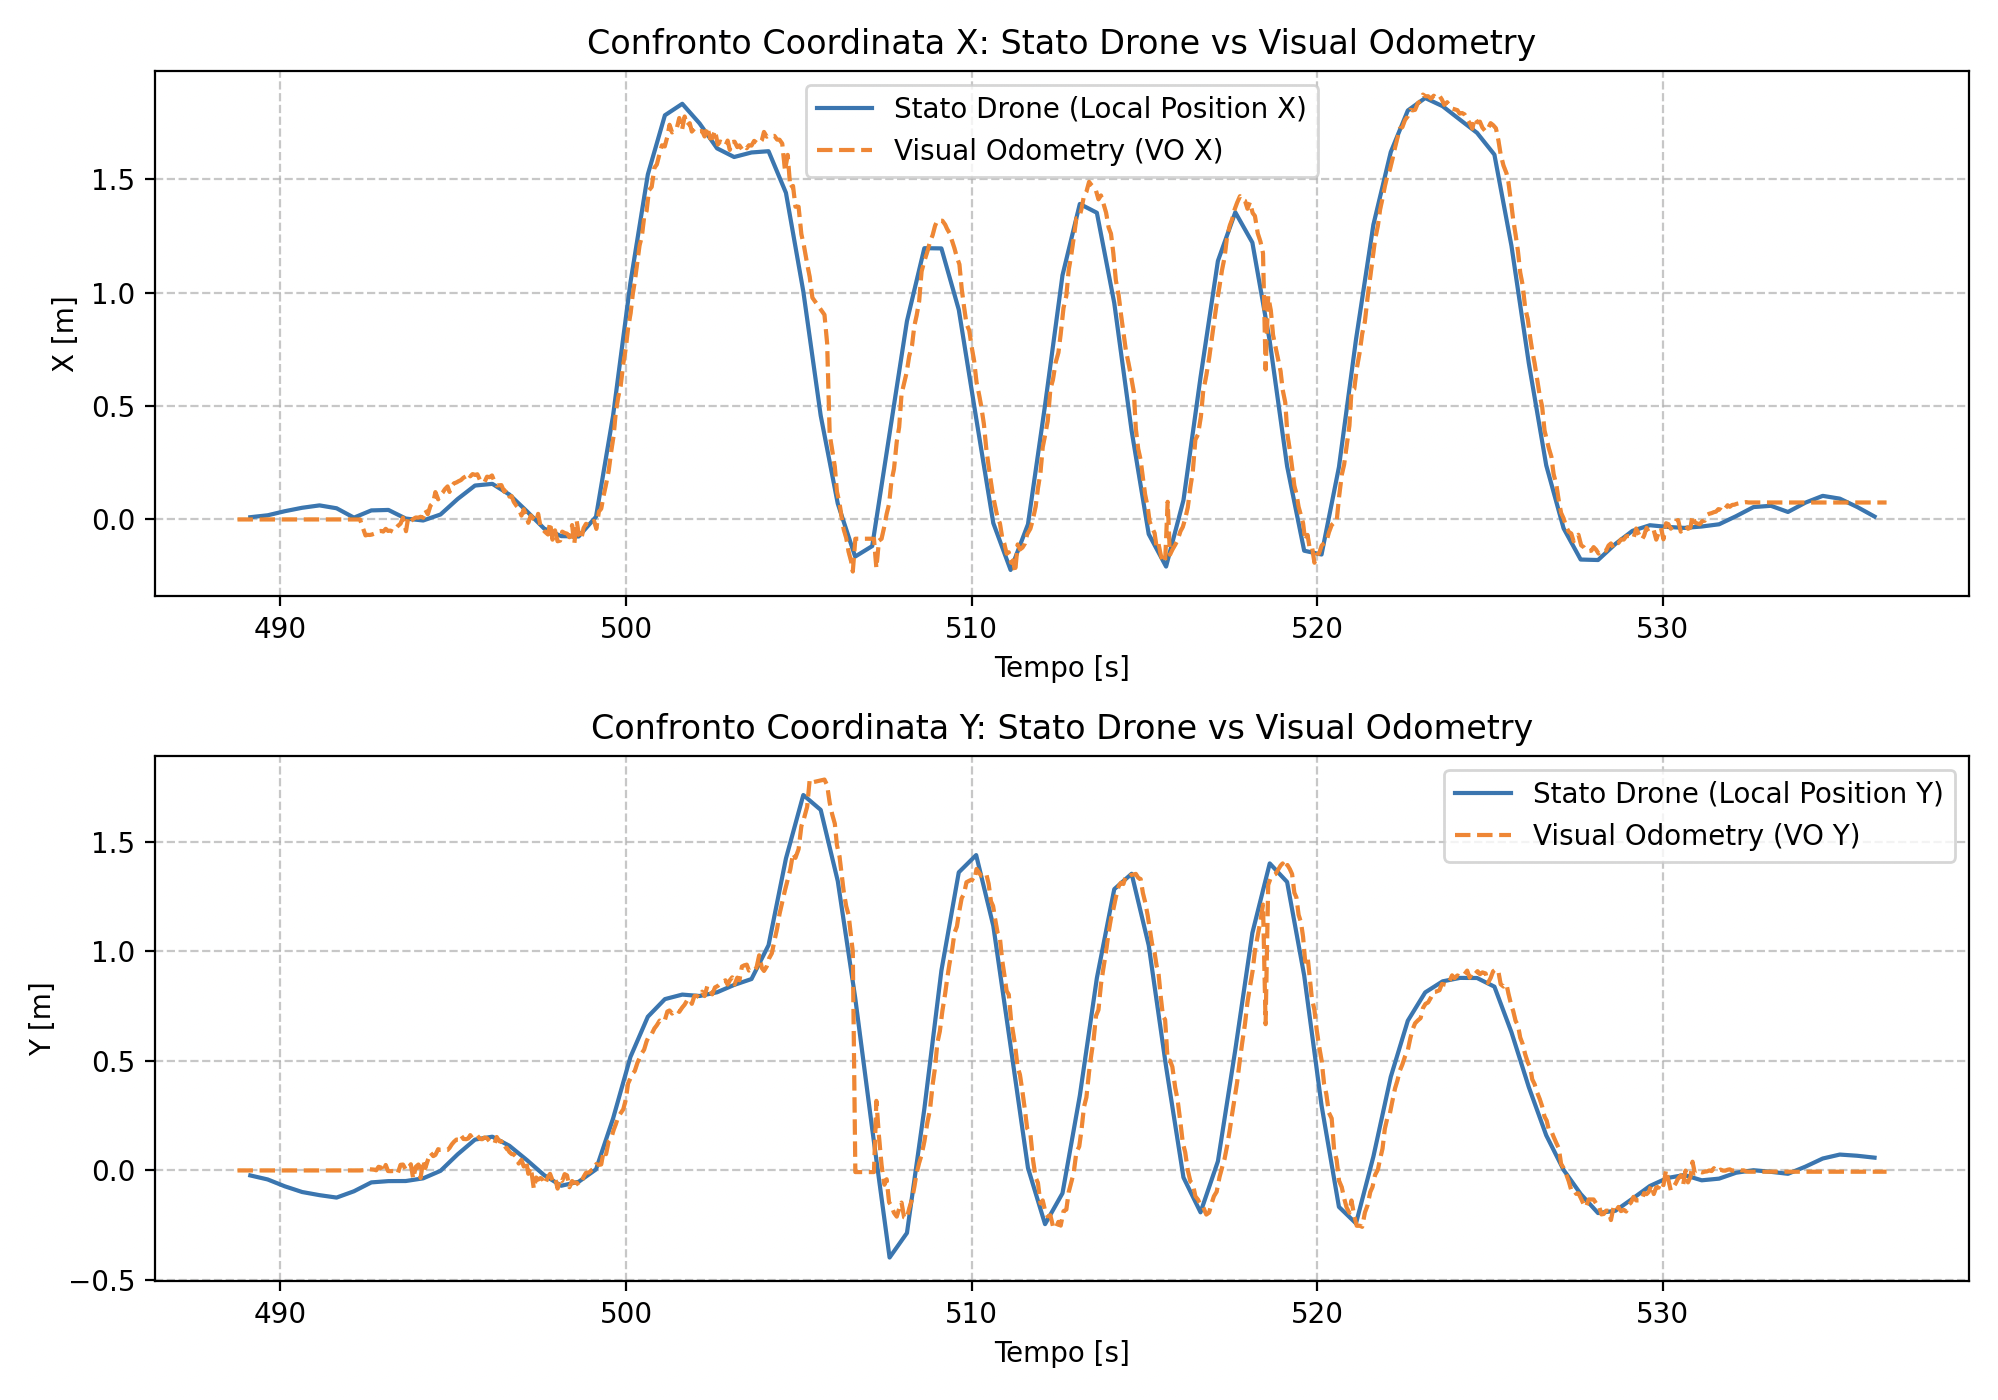
\includegraphics[width = 1\textwidth, trim={0 0 0 0}, clip]{immagini/real_xy.png}
	\caption{Grafico log di volo reale che confronta le coordinate XY della VO e lo stato nel filtro di Kalman.}
	\label{fig:real_xy}
\end{figure}
Mentre per quanto riguarda la coordinata Z (Fig. \ref{fig:real_z}), anche qui si è ottenuto un ottimo risultato. Si possono fare le stesse considerazioni fatte al simulatore per quanto riguarda il decollo/atterraggio e le oscillazioni presenti durante i movimenti del veivolo.
\begin{figure}[!htbp]
	\centering
	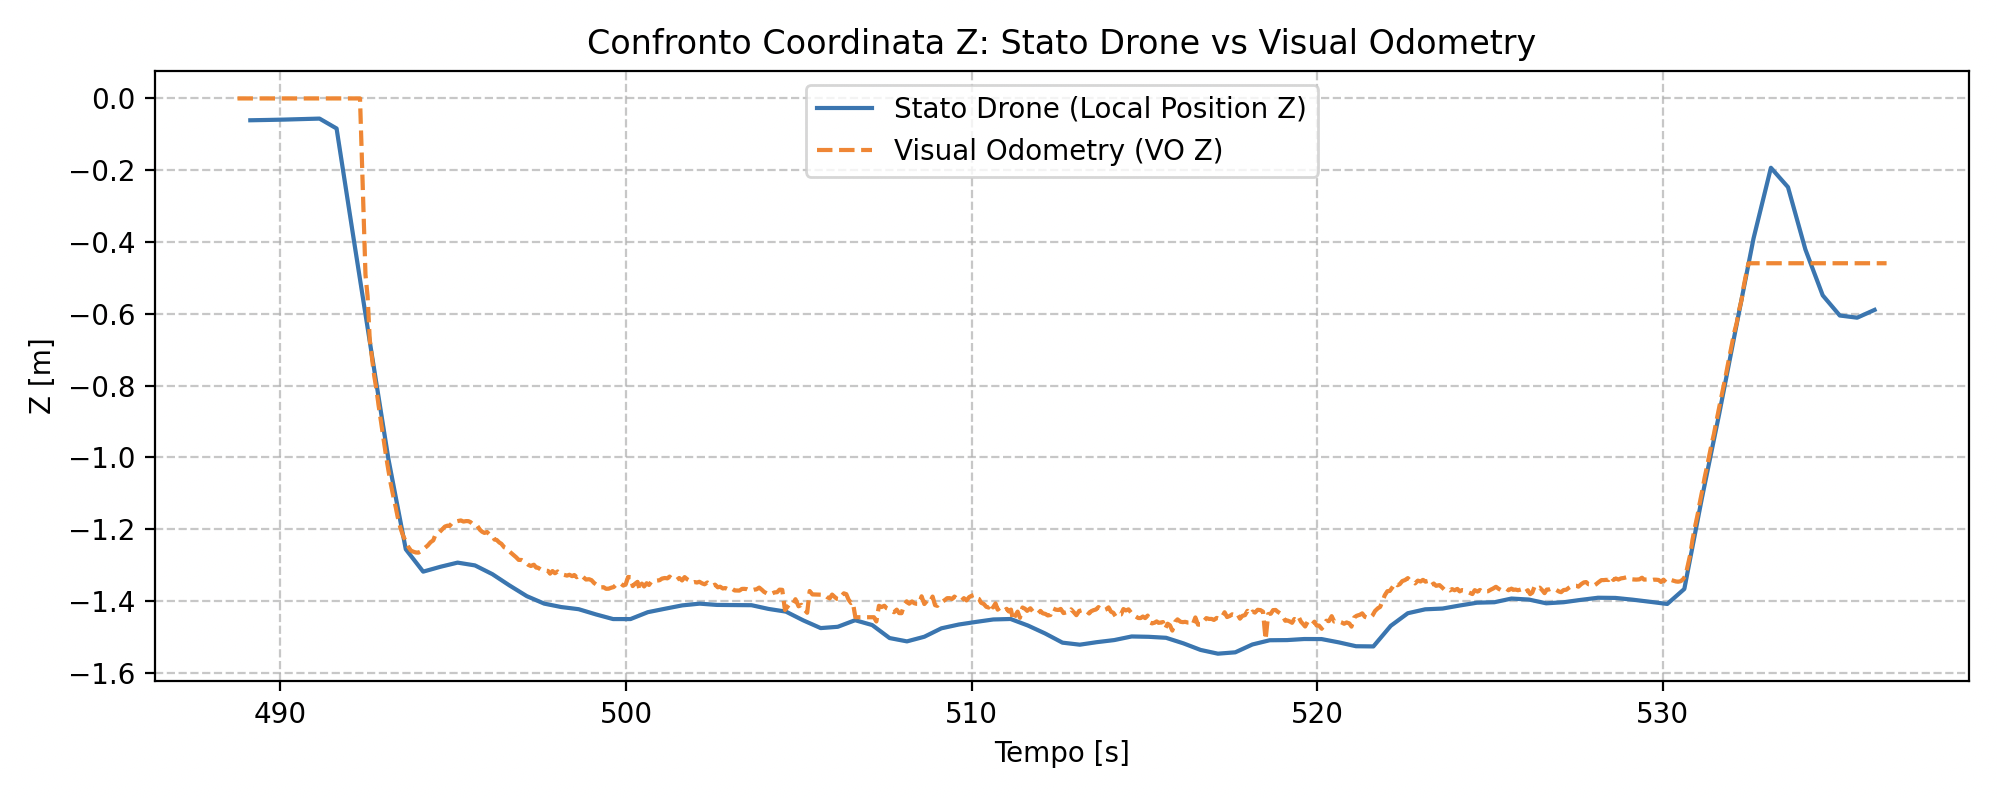
\includegraphics[width = 1\textwidth, trim={0 0 0 0}, clip]{immagini/real_z.png}
	\caption{Grafico log di volo reale che confronta la coordinata Z della VO e lo stato nel filtro di Kalman.}
	\label{fig:real_z}
\end{figure}




analisi coordinate xyz
framerate
analisi cpu, memoria,...
ci sta mettere dei paragrafi: analisi posa, analisi posizione,...